\chapter{Post-Exploitation}
\markboth{Post-Exploitation}{}

\section{Privilege Escalation}
Ora che è stato ottenuto l'accesso al sistema, il prossimo passo è quello di ottenere quanti più privilegi possibile.

\subsection{Fallimento delle strategie automatizzate}
Dal momento che la suite \emph{Metasploit} non ha dato i risultati sperati, ovviamente non è possibile utilizzare i moduli \emph{post} in quanto non è stato possibile generare una sessione. Quindi non potendo utilizzare questo strumento e non avendo trovato vulnerabilità del sistema nei report, si è deciso di continuare con l'analisi manuale
\subsection{Privilege Escalation orizzontale}
Dalla sessione \emph{SSH} dell'utente \textbf{mbrown}, un primo tentativo che è possibile effettuare è provare a cambiare utente sfruttando le password scoperte in precedenza. Utilizzando il comando \texttt{su} su entrambi gli utenti, il risultato è il seguente:
\begin{figure}[h]
    \begin{subfigure}{0.5\textwidth}
        \hspace{0.25\textwidth}
        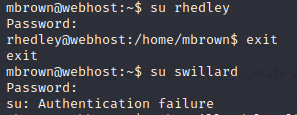
\includegraphics[width=0.5\textwidth]{capitoli/figure/su-users.png}
        \caption{Risultato cambio utente con \texttt{su}}
        \label{fig:su-users}
    \end{subfigure}
    \begin{subfigure}{0.5\textwidth}
        \hspace{0.05\textwidth}
        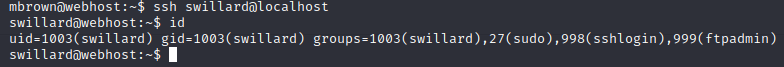
\includegraphics[width=0.9\textwidth]{capitoli/figure/su-users-ssh.png}
        \caption{Cambio utente con \emph{SSH}}
        \label{fig:su-users-ssh}
    \end{subfigure}
    \caption{Risultati cambio utente}
    \label{fig:su}
\end{figure}

Il cambio utente con \textbf{rhedley} ha successo (confermando anche l'esattezza della password) mentre con \textbf{swillard} non si ha successo (la password potrebbe non essere quella). Tuttavia un tentativo \emph{creativo} per provare a cambiare utente, come mostrato in Figura \ref{fig:su-users-ssh}, consiste nel provare a cambiare utente tramite \emph{SSH} e non solo questo tentativo ha successo ma non richiede nemmeno la password dell'utente.\\
Per quanto riguarda \emph{FTP}, con l'utente \textbf{rhedley} si ha ancora una volta successo, mentre con l'utente \textbf{swillard}, di nuovo, non si ha successo.

\subsection{Scoperta di un backup}
Ritornando per un attimo alla shell di \textbf{mbrown}, dalle informazioni recuperate in precedenza sappiamo che esiste un \textbf{backup} sul server. Per cui quello che si può fare è cercare questo backup all'interno del filesystem. Per cercarlo si può usare il comando \texttt{find} grazie al quale possiamo effettuare una ricerca in tutto il filesystem. Immaginando che il nome del backup contenga proprio la parola \emph{backup}, si può lanciare il seguente comando:
\begin{lstlisting}[language=bash]
    find / backup 2>/dev/null | grep backup
\end{lstlisting}
dove con \texttt{2>/dev/null} si evita la stampa degli errori e con \texttt{grep} mostriamo a schermo solo i path che contengono effettivamente la parola \emph{backup}.

Una volta eseguito il comando, il risultato è il seguente:
\begin{figure}[h]
    \centering
    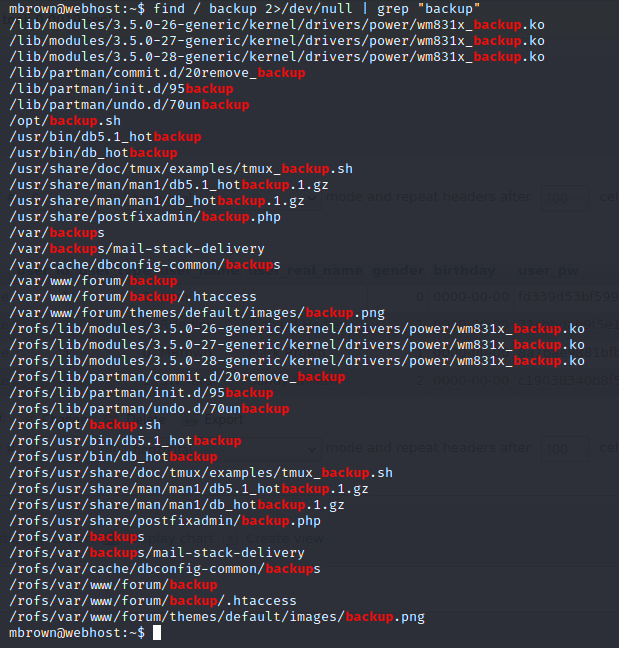
\includegraphics[width=0.4\textwidth]{capitoli/figure/find-backup.png}
    \caption{Output del comando \texttt{find}}
    \label{fig:find-backup}
\end{figure}

Dal risultato ottenuto salta subito all'occhio il percorso \textbf{\texttt{/opt/backup.sh}}, che potrebbe essere proprio lo script utilizzato per effettuare il backup.

\subsection{Decifratura del backup}
Provando a leggere il file come utente \textbf{mbrown} porta ad un \emph{permesso negato} è quindi necessario cambiare utente con, ad esempio, \textbf{rhedley}. La lettura del file porta al seguente risultato:

\begin{figure}[h]
    \centering
    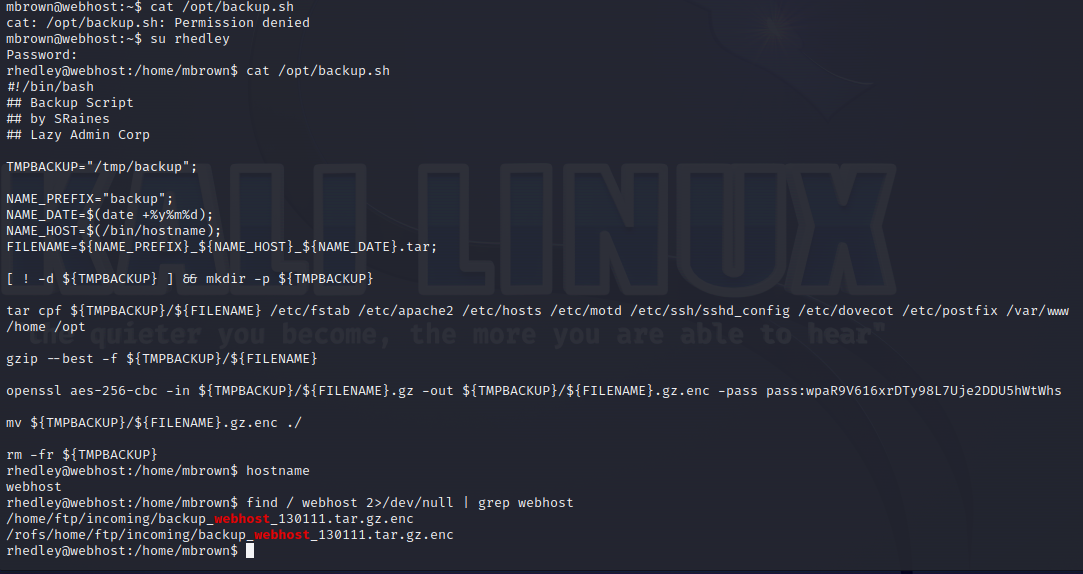
\includegraphics[width=0.7\textwidth]{capitoli/figure/backup-cat.png}
    \caption{Contenuto di \emph{backup.sh} e localizzazione del file di backup}
    \label{fig:backup-cat}
\end{figure}

Come si può notare, è proprio lo script utilizzato per effettuare il backup e, inoltre, questo è cifrato con una chiave che però è stata lasciata in chiaro proprio all'interno dello script. Ovviamente, lanciando lo stesso comando specificando l'opzione \texttt{-d} e il nome del backup, quello che succede è che decifriamo il backup. Una volta compreso il funzionamento dello script e il nome utilizzato per salvarlo, basta semplicemente specificare quello come nome di input e come nome di output si è scelto semplicemente \textbf{decrypted.tar.gz}. Quindi, il file ottenuto dalla decifratura è un archivio \texttt{.tar.gz} e, per evitare di lavorare direttamente sulla macchina, si effettua il login tramite \emph{FTP} con l'utente \textbf{rhedley} e si effettua il download del file che si trovava nel path \emph{ftp/incoming} (come visto dallo script), come mostrato di seguito:
\begin{figure}[h]
    \centering
    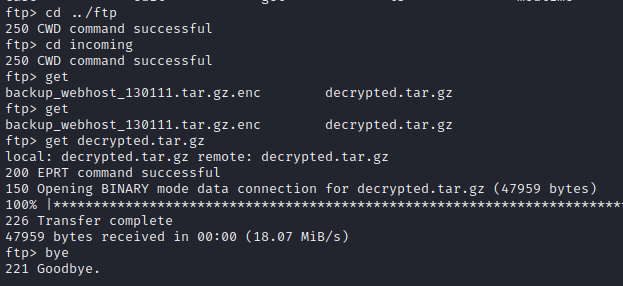
\includegraphics[width=0.7\textwidth]{capitoli/figure/ftp-rhedley-decrypted.png}
    \caption{Download del backup tramite \emph{FTP}}
    \label{fig:ftp-decrypted}
\end{figure}

Una volta effettuato il download, l'archivio viene estratto prima tramite \texttt{gzip} e successivamente tramite \texttt{tar}, come mostrato di seguito:
\begin{figure}[h]
    \begin{subfigure}{0.5\textwidth}
        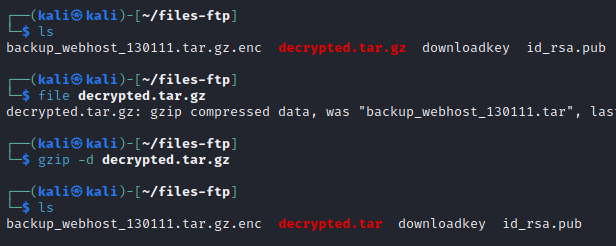
\includegraphics[width=1\textwidth]{capitoli/figure/decrypted-1.png}
        \caption{Estrazione con \texttt{gzip}}
        \label{fig:decrypted-1}
    \end{subfigure}
    \begin{subfigure}{0.5\textwidth}
        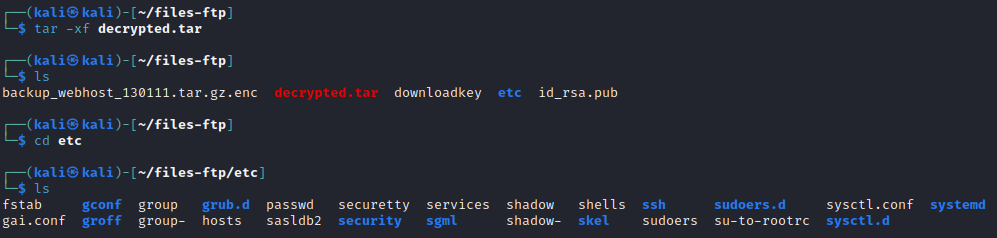
\includegraphics[width=1\textwidth]{capitoli/figure/decrypted-2.png}
        \caption{Estrazione con \texttt{tar} e visita del contenuto}
        \label{fig:decrypted-2}
    \end{subfigure}
    \caption{Estrazione e contenuto del backup}
    \label{fig:decrypted}
\end{figure}

Come si può vedere nella Figura \ref{fig:decrypted-2}, il contenuto del backup è il contenuto della cartella \emph{/etc} e, visualizzando il contenuto, si nota la presenza dei file \textbf{passwd} \textbf{shadow}.

\subsection{Cracking delle password trovate all'interno del backup}
Utilizzando il tool \texttt{unshadow}, si possono ricostruire gli hash presenti all'interno dei due file e salvarli all'interno di un file che è stato chiamato \textbf{password}. Successivamente l'output si può dare in pasto ad un tool di \emph{Offline Password Cracking}, come mostrato di seguito:
\begin{figure}[h]
    \begin{subfigure}{0.5\textwidth}
        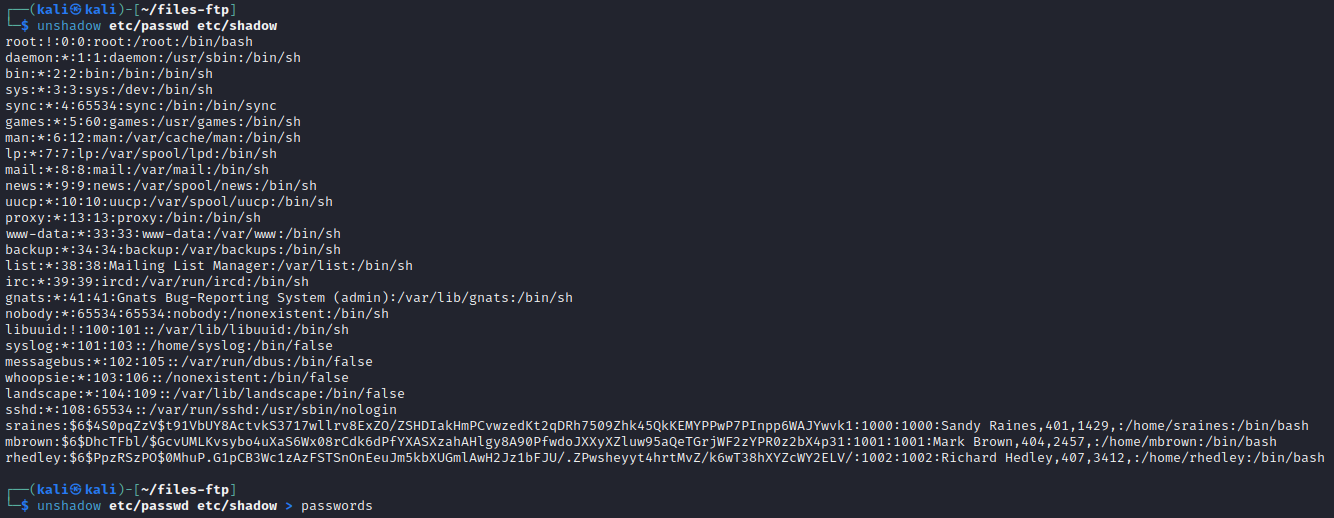
\includegraphics[width=1\textwidth]{capitoli/figure/unshadow.png}
        \caption{Ricostruzione degli hash delle password}
        \label{fig:unshadow}
    \end{subfigure}
    \begin{subfigure}{0.5\textwidth}
        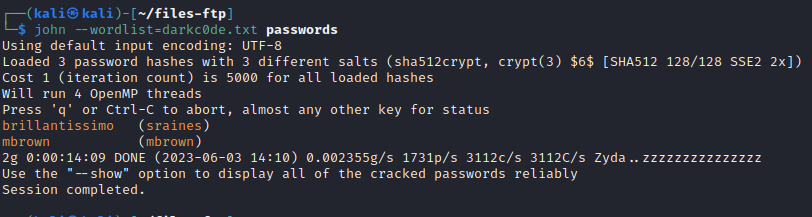
\includegraphics[width=1\textwidth]{capitoli/figure/passwd-john-recovered.png}
        \caption{Cracking delle password con \texttt{john}}
        \label{fig:john}
    \end{subfigure}
    \caption{Recupero della password di un nuovo utente}
    \label{fig:password-cracking}
\end{figure}

Per il cracking sono state utilizzate varie wordlist, ma l'unica che ha dato un risultato concreto è stata \textbf{darkc0de}.\\
A quanto sembra è stata recuperata sia la password di \textbf{mbrown} che di un nuovo utente chiamato \textbf{sraines}, tuttavia la password di \textbf{mbrown} non è quella recuperata e, inoltre, non esiste nessun utente \textbf{sraines}, come illustrato di seguito:

\begin{figure}[h]
    \centering
    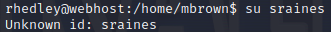
\includegraphics[width=0.5\textwidth]{capitoli/figure/sraines.png}
    \caption{Tentativo di cambio utente con \textbf{sraines}}
    \label{fig:sraines}
\end{figure}

\subsection{Privilege Escalation Verticale}
L'ultimo tentativo che si può fare è quello di tentare entrambe le password per gli unici due utenti di cui ancora non sappiamo la password: \textbf{mbrown} e \textbf{swillard}. Sorprendentemente, la password \textbf{brillantissimo} è proprio la password di \textbf{swillard} e, adesso, possiamo effettuare il login come quest'ultimo senza utilizzare l'approccio dell'\emph{SSH}. A questo punto, per capire il prossimo passo da eseguire bisogna capire quale sia la password dell'utente \textbf{root} o di un \textbf{sudoer}. Per visualizzare la lista dei \emph{sudoer} basta leggere il file \emph{/etc/groups} e vedere quali utenti hanno il gruppo \texttt{sudo}. L'output della lettura, effettuata utilizzando il filtro \texttt{grep} è il seguente:
\begin{figure}[h]
    \centering
    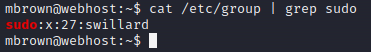
\includegraphics[width=0.5\textwidth]{capitoli/figure/sudo.png}
    \caption{Lista dei \emph{sudoer}}
    \label{fig:sudo}
\end{figure}

A quanto pare l'unico utente con i permessi di \texttt{sudo} è proprio \textbf{swillard}, di cui abbiamo appena scoperto la password. A questo punto, effettuando il login come quest'ultimo ed eseguendo il comando \texttt{sudo su} quello che si ottiene è che si diventa utente \textbf{root}, come mostrato di seguito:
\begin{figure}[h]
    \centering
    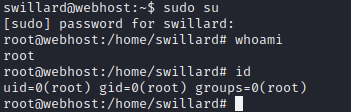
\includegraphics[width=0.6\textwidth]{capitoli/figure/root.png}
    \caption{Cambio ad utente \textbf{root}}
    \label{fig:root}
\end{figure}

Così facendo, è stato possibile effettuare una violazione completa del sistema assumendo pieno controllo sulla macchina.
\section{Maintaining Access}

\subsection{Creazione della backdoor}


\subsection{Trasferimento della backdoor sull'asset}

\subsection{Abilitazione della backdoor}

\subsection{Impossibilità di testing della backdoor}